\chapter{Preliminary Evaluation}\label{C:evaluation}

The result is from analysing the Whiley benchmark. The pipeline used is a bloom filter into a list spectra with Levenshtein distance metric and finally into calling context spectra with Levenshtein distance metric. The Figure \ref{fig:similiartests} shows the current state of the GUI, although limited it allows the user to see the results from a pipeline visually rather than through a text file. In the example, the potential redundant test cases in comparison to Byte\_Valid\_5 are being examined. This shows that Byte\_Valid\_6, 8 and 9 are potential redundant tests that require further examination.

\begin{figure}[h]
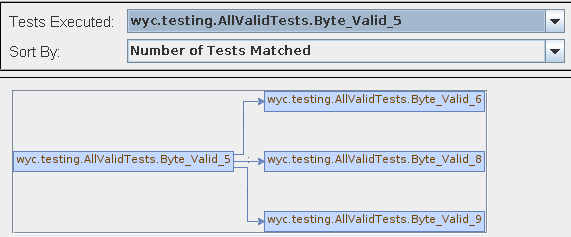
\includegraphics[width=\textwidth]{model24.png}
\caption{GUI showing similar test cases}
\label{fig:similiartests}
\end{figure}

This involves examining the Whiley files which would give insight into how closely related these two tests are. Comparing Byte\_Valid\_5 and Byte\_Valid\_8 in Figure \ref{fig:bytecompare}. It shows that the difference between the tests is the range of j and two additional addition statements. This indicates a high level of redundancy, such that removing Byte\_Valid\_8 could be achieved. This is because if \textit{Any.toString(i $<<$ j)} executed without error, then \textit{Any.toString(i $<<$ (j + 1))} would as well as long as the addition is bug free. Since this test is not designed to test addition, we can assume it will work. Although this shows that this is indeed a redundant test, comparing Byte\_Valid\_6 and Byte\_Valid\_9 with Byte\_Valid\_5 shows that these two are false positives. A case that Maurer et al. \cite{koochakzadeh2009test} and Robinson et al. \cite{li2008static} described having issues with. To get around this, the idea of weighting was introduced. By running the same pipeline with weighting, it was expected to remove one or both of the false positives. However, it removed neither and gave the same result back for Byte\_Valid\_5 . This shows that the weighting method implemented needs to be improved on to remove these false positives.

\begin{figure}[h]
\textbf{Byte\_Valid\_8}
\begin{lstlisting}
public method main(System.Console sys) -> void:
    for i in constants:
        for j in 0 .. 8:
            sys.out.print(Any.toString(i) ++ " << ")
            sys.out.print("1+" ++ Any.toString(j) ++ " = ")
            sys.out.println(Any.toString(i << (1 + j)))
\end{lstlisting}
\textbf{Byte\_Valid\_5}
\begin{lstlisting}
public method main(System.Console sys) -> void:
    for i in constants:
        for j in 0 .. 9:
            sys.out.print(Any.toString(i) ++ " << ")
            sys.out.print(Any.toString(j) ++ " = ")
            sys.out.println(Any.toString(i << j))
\end{lstlisting}
\caption{Byte\_Valid\_8 Comparison with Byte\_Valid\_5}
\label{fig:bytecompare}
\end{figure}